\chapter{The Real Toolkit: Sequences, Functions, and Equations}

\begin{figure}[ht]       
\centerline{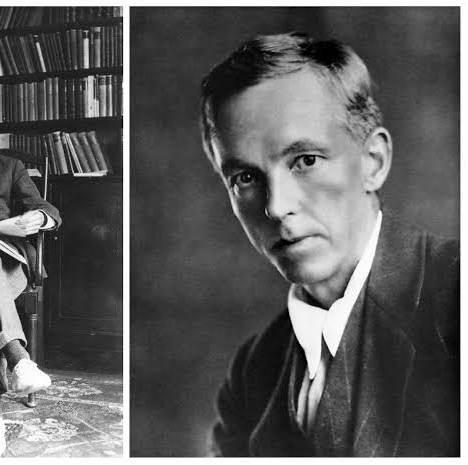
\includegraphics[width=1.0in]{images/hardy2.jpeg}}
\caption*{\small ``A mathematician, like a painter or a poet, is a maker of patterns'' -- \href{https://en.wikipedia.org/wiki/G._H._Hardy}{G. H. Hardy}}
\end{figure}

%\begin{figure}[ht]       
%\centerline{
\includegraphics[width=1.0in]{images/plato2.jpeg}}
%\caption*{\small ``He is unworthy of the name of man who is ignorant of the fact that the diagonal of a square is incommensurable with its side'' -- \href{https://en.wikipedia.org/wiki/Plato}{Plato}}
%\end{figure}

The real numbers are more than a continuum filling the gaps left by the rationals—they form a versatile algebraic toolkit for describing change, predicting patterns, and solving practical problems. In this chapter we develop the basic algebra of the reals as it appears in everyday mathematical modelling: from  arithmetic and geometric progressions; from polynomials and their remarkable power of unique interpolation to the curve-fitting techniques that underlie modern data analysis; and from real-valued functions to systems of linear equations that allow us to solve for unknowns in structured ways. Together, these ideas illustrate how the algebra of the real numbers becomes a unifying language for patterns, growth, and relationships in both mathematics and the world around us.

%%%%%%%%%%%%%%%%%%%%%%%%%%%%%%%%%%%%%%%%%%%%%%%%%%%%%%%%%%%%%%
\section{Arithmetic and geometric progressions}
\label{sec:apgp}

Arithmetic and geometric progressions are two of the simplest infinite families
of sequences, and they sit at the gateway between discrete sums and the
idea of limits.  They also provide the first nontrivial examples of
closed-form formulas for sums.

\subsection{Arithmetic progressions (AP)}

\begin{definition}
A sequence $(a_n)$ is an \emph{arithmetic progression} if the difference between
consecutive terms is constant.  That is, there exists a real number $d$
such that
\[
a_{n+1}-a_n=d\quad\text{for all }n\ge 1.
\]
The number $d$ is called the \emph{common difference}.
\end{definition}

Hence an AP has the form
\[
a,\ a+d,\ a+2d,\ \dots,\ a+(n-1)d,\ \dots
\]
and the $n$-th term is
\[
a_n=a+(n-1)d.
\]

\subsubsection*{Sum of the first $n$ terms: a double-counting derivation}

Let
\[
S_n = a + (a+d) + (a+2d) + \cdots + (a+(n-1)d)
\]
be the sum of the first $n$ terms.

Write the same sum in reverse order:
\[
S_n = (a+(n-1)d) + (a+(n-2)d) + \cdots + (a+d) + a.
\]

Now add these two expressions term-by-term.  Each pair adds to the same value\footnote{This ``pairing'' trick is often attributed to the young \href{https://en.wikipedia.org/wiki/Carl_Friedrich_Gauss}{Gauss}, who is said
to have summed $1+2+\cdots+100$ instantly by noticing that $1+100=2+99=\cdots=101$.}:
\[
\bigl(a+(k-1)d\bigr) + \bigl(a+(n-k)d\bigr)=2a+(n-1)d.
\]
There are $n$ such pairs, so
\[
2S_n = n\bigl(2a+(n-1)d\bigr).
\]
Therefore,
\[
\boxed{\displaystyle
S_n = \frac{n}{2}\bigl(2a+(n-1)d\bigr)
     = \frac{n}{2}\,(a_1+a_n).
}
\]

\begin{example}[Sum of the first $n$ natural numbers]
Here $a=1$ and $d=1$, so
\[
S_n=\frac{n}{2}(2+(n-1))=\frac{n(n+1)}{2}.
\]
\end{example}

\begin{example}[Sum of the first $n$ odd numbers]
The odd numbers form an AP:
\[
1,3,5,\dots,(2n-1),
\]
with $a=1$, $d=2$. Thus
\[
S_n=\frac{n}{2}\bigl(2\cdot 1+(n-1)\cdot 2\bigr)
=\frac{n}{2}(2n)=n^2.
\]
So the sum of the first $n$ odd numbers is $n^2$.
\end{example}

\subsection{Geometric progressions (GP)}

\begin{definition}
A sequence $(g_n)$ is a \emph{geometric progression} if the ratio between
consecutive terms is constant.  That is, there exists a real number $r$
such that
\[
\frac{g_{n+1}}{g_n}=r\quad\text{for all }n\ge 1,
\]
provided $g_n\neq 0$.
The number $r$ is called the \emph{common ratio}.
\end{definition}

A GP has the form
\[
a,\ ar,\ ar^2,\ \dots,\ ar^{n-1},\ \dots
\]
and the $n$-th term is
\[
g_n=ar^{n-1}.
\]

\subsubsection*{Sum of the first $n$ terms}

Let
\[
S_n = a + ar + ar^2 + \cdots + ar^{n-1}.
\]
Multiply both sides by $r$:
\[
rS_n = ar + ar^2 + \cdots + ar^{n}.
\]
Subtract:
\[
S_n - rS_n = a - ar^{n}.
\]
Hence
\[
(1-r)S_n = a(1-r^n),
\]
and therefore, if $r\neq 1$,
\[
\boxed{\displaystyle
S_n = a\,\frac{1-r^{n}}{1-r}.
}
\]
When $r=1$, the GP is constant and $S_n=na$.

\subsubsection*{Infinite geometric series}

If $|r|<1$, then $r^n\to 0$ as $n\to\infty$, so
\[
S_\infty
=\lim_{n\to\infty} S_n
=\lim_{n\to\infty} a\,\frac{1-r^n}{1-r}
=\frac{a}{1-r}.
\]
Thus
\[
\boxed{\displaystyle
a+ar+ar^2+\cdots = \frac{a}{1-r}\quad (|r|<1).
}
\]

This is one of the earliest places where limits naturally enter: an infinite
sum makes sense only because the partial sums converge.


\begin{example}[Zeno's geometric series]
\[
\frac12+\frac14+\frac18+\cdots
\]
is a GP with $a=\tfrac12$ and $r=\tfrac12$, so
\[
S_\infty = \frac{1/2}{1-1/2}=1.
\]
This is exactly the mathematical resolution of Zeno’s paradox.
\end{example}

\begin{example}[A repeating decimal as a GP]
\[
0.\overline{3}=0.3+0.03+0.003+\cdots
\]
is a GP with $a=0.3$ and $r=0.1$. Hence
\[
0.\overline{3} = \frac{0.3}{1-0.1}=\frac{0.3}{0.9}=\frac13.
\]
\end{example}

\subsection*{Remarks}

\begin{itemize}
    \item AP sums grow \emph{quadratically} in $n$ when $d\neq 0$,
          reflecting linear increments.
    \item GP sums grow \emph{exponentially} in $n$ when $|r|>1$,
          reflecting multiplicative change.
    \item The infinite GP formula is the first rigorous example of
          a convergent infinite series, and is a key bridge to calculus.
\end{itemize}

\section{Polynomials}

Polynomials are among the most fundamental objects in algebra.  They form
a rich class of functions that are easy to compute with, easy to
approximate, and powerful enough to model a wide variety of phenomena.
In this section we introduce the basic theory of polynomials, discuss the
unique interpolation theorem, and show how polynomials naturally arise in
curve fitting and other applications.

\subsection{Definition and degree}

A \emph{polynomial} over the real numbers is a function of the form
\[
P(x) = a_0 + a_1 x + a_2 x^2 + \cdots + a_n x^n,
\]
where $a_0,a_1,\dots,a_n\in\mathbb{R}$ and $n$ is a nonnegative integer.
The number $n$ is the \emph{degree} of the polynomial (provided $a_n\neq 0$).

\begin{itemize}
    \item A polynomial of degree $0$ is a constant function.
    \item A polynomial of degree $1$ is a linear function. It gives the equation of a straight line.
    \item A polynomial of degree $2$ is a quadratic function.
    \item A polynomial of degree $3$ is a cubic function, and so on.
\end{itemize}

The set of all polynomials with real coefficients is denoted by
$\mathbb{R}[x]$.  Polynomials are defined everywhere on $\mathbb{R}$.  They also satisfy the useful property that if
\[
P(x)=0\quad\text{for infinitely many distinct }x\in\mathbb{R},
\]
then $P$ must be the zero polynomial.  This is called the
\emph{identity theorem for polynomials}.

\subsection{Basic algebraic properties}

Polynomials can be added and multiplied term-by-term, following the same
rules as with ordinary algebraic expressions.  Here we illustrate both
operations with simple examples.

\[
\deg(P+Q)\le\max(\deg P,\deg Q),\qquad
\deg(PQ)=\deg P+\deg Q,
\]
unless cancellation occurs in the leading terms.

\subsubsection*{Polynomial addition}

Let
\[
P(x)=3x^3 - 2x + 5,\qquad
Q(x)=4x^2 + x - 1.
\]
To compute $P(x)+Q(x)$, we combine like terms:
\[
\begin{aligned}
P(x)+Q(x)
&= (3x^3) + (4x^2) + (-2x+x) + (5-1) \\
&= 3x^3 + 4x^2 - x + 4.
\end{aligned}
\]
Thus
\[
\boxed{\,P(x)+Q(x)=3x^3 + 4x^2 - x + 4.\,}
\]

\subsubsection*{Polynomial multiplication}

Let
\[
A(x)=2x^2 - 3x + 1,\qquad
B(x)=x - 4.
\]
Multiplying out (using distributivity):
\[
\begin{aligned}
A(x)B(x)
&=(2x^2)(x) + (2x^2)(-4)
 +(-3x)(x)+(-3x)(-4)
 +(1)(x)+(1)(-4) \\
&= 2x^3 - 8x^2 - 3x^2 + 12x + x -4.
\end{aligned}
\]
Now combine like terms:
\[
\begin{aligned}
A(x)B(x)
&= 2x^3 - 11x^2 + 13x - 4.
\end{aligned}
\]
So
\[
\boxed{\,A(x)B(x)=2x^3 - 11x^2 + 13x - 4.\,}
\]

\subsection{The decimal system as a polynomial representation}

Every finite decimal expansion
\[
d_k d_{k-1} \cdots d_1 d_0
\]
represents a number that can be interpreted as a polynomial in~$10$:
\[
d_k 10^{k} + d_{k-1} 10^{k-1} + \cdots + d_1 10 + d_0.
\]
In this sense, the decimal numeral system is simply a \emph{polynomial in the base~$10$}.

\begin{example}
\begin{enumerate}
\item A whole number:
\[
374 = 3\cdot 10^2 + 7\cdot 10^1 + 4\cdot 10^0.
\]
\item A larger number:
\[
5{,}182
= 5\cdot 10^3 + 1\cdot 10^2 + 8\cdot 10 + 2.
\]
\item A decimal (fractional) number:
For digits after the decimal point, we use negative powers of~10:
\[
46.327
= 4\cdot 10^1
+ 6\cdot 10^0
+ 3\cdot 10^{-1}
+ 2\cdot 10^{-2}
+ 7\cdot 10^{-3}.
\]
\end{enumerate}
\end{example}
\medskip

Thus every decimal numeral is nothing more than a polynomial expression
in the base~$10$ with coefficients drawn from $\{0,1,\dots,9\}$.
This viewpoint is fundamental in computer science (base~2),
engineering (base~16), and number theory (general base-$b$ expansions).

\begin{exercise}
Explain the junior school algorithm for integer multiplication in terms of polynomial multiplications. Explain how is this repeated addition?
\end{exercise}

\subsection{The unique interpolation theorem}

One of the most remarkable facts about polynomials is that they can be
used to fit any finite collection of data points with a unique polynomial
of sufficiently small degree.

\begin{theorem}[Unique Interpolating Polynomial]
Let $(x_0,y_0), (x_1,y_1), \dots, (x_n,y_n)$ be $n\!+\!1$ data points with
\[
x_i \neq x_j \quad \text{whenever } i\neq j.
\]
Then there exists a polynomial $P(x)$ of degree at most $n$ such that
\[
P(x_i)=y_i \quad \text{for all } i=0,1,\dots,n,
\]
and this polynomial is unique.
\end{theorem}

\begin{proof}
We prove existence and uniqueness.

\subsubsection*{Existence (\href{https://en.wikipedia.org/wiki/Joseph-Louis_Lagrange}{Lagrange} construction)}
For each $k\in\{0,1,\dots,n\}$ define the \emph{Lagrange basis polynomial}
\[
L_k(x)
=
\prod_{\substack{0\le j\le n \\ j\neq k}}
\frac{x-x_j}{x_k-x_j}.
\]
This is well-defined because $x_k-x_j\neq 0$ for $j\neq k$.

\medskip
\noindent
\textbf{Claim 1.} For all $i,k\in\{0,\dots,n\}$,
\[
L_k(x_i)=\delta_{ik}=
\begin{cases}
1,& i=k,\\
0,& i\neq k.
\end{cases}
\]

\noindent
\emph{Proof of Claim 1.}
If $i=k$, then every factor in the product equals
\[
\frac{x_k-x_j}{x_k-x_j}=1,
\]
so $L_k(x_k)=1$.
If $i\neq k$, then the product defining $L_k$ contains the factor with
$j=i$, namely
\[
\frac{x_i-x_i}{x_k-x_i}=0,
\]
so $L_k(x_i)=0$.  This proves the claim. \hfill $\square$

\medskip
Now define
\[
P(x)=\sum_{k=0}^n y_k\,L_k(x).
\]
Each $L_k$ is a polynomial of degree $n$ (a product of $n$ linear factors),
so $P$ is a polynomial of degree at most $n$.

Evaluate $P$ at each interpolation point $x_i$:
\[
P(x_i)
=
\sum_{k=0}^n y_k\,L_k(x_i)
=
\sum_{k=0}^n y_k\,\delta_{ik}
=
y_i.
\]
Hence $P$ interpolates all the given data.  Existence is proved.

\subsubsection*{Uniqueness}
We need one standard fact.

\medskip
\noindent
\textbf{Lemma.} A nonzero polynomial of degree at most $n$ can have at most
$n$ distinct real roots.

\noindent
\emph{Proof of Lemma.}
We proceed by induction on $n$.
For $n=0$, a nonzero constant polynomial has no roots.  
Assume the statement true for degree at most $n-1$.
Let $Q$ be a nonzero polynomial of degree at most $n$ with a root $a$.
Then $(x-a)$ divides $Q(x)$, so
\[
Q(x)=(x-a)R(x)
\]
for some polynomial $R$ of degree at most $n-1$.
Any root of $Q$ different from $a$ must be a root of $R$, and by the
induction hypothesis $R$ has at most $n-1$ distinct roots.  
Thus $Q$ has at most $n$ distinct roots in total. \hfill $\square$

\medskip
Now suppose $P$ and $Q$ are two polynomials of degree at most $n$ both
interpolating the data:
\[
P(x_i)=Q(x_i)=y_i \quad \text{for all } i=0,\dots,n.
\]
Consider their difference
\[
R(x)=P(x)-Q(x).
\]
Then $\deg R\le n$, and
\[
R(x_i)=P(x_i)-Q(x_i)=0 \quad \text{for all } i=0,\dots,n.
\]
So $R$ has at least $n\!+\!1$ distinct roots.  
By the lemma, the only polynomial of degree at most $n$ that can have
$n\!+\!1$ roots is the zero polynomial.  Hence $R\equiv 0$, i.e.
\[
P(x)=Q(x)\quad\text{for all }x.
\]
Therefore the interpolating polynomial is unique.
\end{proof}
\subsubsection*{A simple example}

Given
\[
(0,1),\qquad (1,2),\qquad (2,5),
\]
there is a unique quadratic polynomial through these points.  Using the
Lagrange formula,
\[
P(x)=1\cdot \frac{(x-1)(x-2)}{(0-1)(0-2)}
      +2\cdot \frac{(x-0)(x-2)}{(1-0)(1-2)}
      +5\cdot \frac{(x-0)(x-1)}{(2-0)(2-1)}.
\]
Simplifying yields
\[
P(x)=x^2+1.
\]

\subsection{Polynomials and curve fitting}

Interpolation provides an exact polynomial passing through given data,
but  we often only have noisy measurements or more data points
than we want the degree of the polynomial to match.  
In practice, measured data points rarely lie exactly on a straight line, a
quadratic curve, or any simple mathematical model.  We therefore need a way
to choose a ``best'' curve that captures the overall trend of the data,
without requiring a perfect fit to every point.  The most widely used
approach is the \emph{method of least squares}, which selects the curve
whose predicted values come, on average, as close as possible to the
observations.

The idea is simple to state: among all candidate lines or curves, choose the
one that \emph{minimises the total squared error}
\[
\sum_{i=1}^n (y_i - P(x_i))^2,
\]
where $P(x)$ is the model we want to fit.  Squaring the errors penalises
large deviations more strongly and leads to a unique, stable solution.
Although the derivation is not required here, the resulting formulas give
clean, explicit expressions for the best-fitting straight line or quadratic
polynomial.

Historically, the method was developed by \href{https://en.wikipedia.org/wiki/Carl_Friedrich_Gauss}{Carl Friedrich Gauss} in
the early 19th century in his work on determining planetary orbits from
noisy astronomical measurements.  Gauss famously used least squares to
recover the orbit of the asteroid \emph{Ceres} in~1801, demonstrating that
the best-fitting curve---in the least-squares sense---provides the most
reliable prediction from imperfect data.  Today the same principle forms the
basis of regression, statistical modelling, and modern machine learning.

We will not describe his methods in these notes and leave it for a future course. In what follows we give some examples to illustrate the use of least squares approximation.

\begin{example}[Linear Fit Example (Economics): Wage vs.\ Experience]

A common empirical observation in labour economics is that, over an early
career window, wages rise approximately linearly with experience.
Suppose we measure monthly wage $W$ (in thousand rupees) for workers with
different years of experience $x$:

\begin{center}
\begin{tabular}{c|cccccc}
Experience $x$ (years) & 0 & 2 & 4 & 6 & 8 & 10\\ \hline
Wage $W$ (\rupee'000/month)  & 30 & 38 & 46 & 55 & 63 & 70
\end{tabular}
\end{center}

\begin{figure}[h]
\centering
\begin{tikzpicture}[scale=0.5]

% Axes
\draw[->] (0,0) -- (11,0) node[right] {Experience $x$ (years)};
\draw[->] (0,0) -- (0,8) node[above] {Wage (\rupee'000/month)};

% x ticks
\foreach \x in {0,2,4,6,8,10} {
  \draw (\x,0) -- (\x,-0.12);
  \node[below] at (\x,-0.18) {\x};
}

% y ticks: 0 to 80k in 10k increments
\foreach \y/\lab in {0/0,1/10,2/20,3/30,4/40,5/50,6/60,7/70,8/80} {
  \draw (0,\y) -- (-0.12,\y);
  \node[left] at (-0.18,\y) {\lab};
}

% Data points (actual wages divided by 10)
\fill (0,3.0) circle (2pt);   % 30k
\fill (2,3.8) circle (2pt);   % 38k
\fill (4,4.6) circle (2pt);   % 46k
\fill (6,5.5) circle (2pt);   % 55k
\fill (8,6.3) circle (2pt);   % 63k
\fill (10,7.0) circle (2pt);  % 70k

% Best-fit line: W = 4.06x + 30.05   (in thousands)
% y = (W/10) = 0.406x + 3.005
\draw[thick, dashed] (0,3.005) -- (10,7.065);

% Legend
%\begin{scope}[shift={(6.0,7.0)}]
%  \fill (0,0) circle (2pt);
%  \node[right] at (0.2,0) {\small data};
%
%  \draw[thick, dashed] (0,-0.6) -- (1.0,-0.6);
%  \node[right] at (1.2,-0.6) {\small least-squares line};
%\end{scope}

\end{tikzpicture}

\caption{Wage vs.\ experience.}
\label{fig:linear-fit}
\end{figure}

We model this by a straight line
\[
W(x) \approx mx + c.
\]
A least--squares calculation gives (See Figure \ref{fig:linear-fit})
\[
m \approx 4.06,\qquad c \approx 30.05,
\]
so the fitted wage equation is
\[
\boxed{\,W(x) \approx 4.06x + 30.05.\,}
\]

\noindent
\textbf{Interpretation.}
The slope means that each additional year of experience raises expected
wage by about \rupee4,060 per month in this range.  The intercept estimates a
starting wage around \rupee30,000 per month.

\end{example}

\begin{example}[Quadratic Fit Example (Economics): Profit vs.\ Output]

In many production settings, profits rise with output at first, but beyond
some point diminishing returns and rising costs reduce profits.  This often
produces a concave (downward-opening) quadratic relationship.

Suppose a firm varies daily output $q$ (in hundreds of units) and observes
profit $\Pi$ (in thousand rupees):

\begin{center}
\begin{tabular}{c|ccccccc}
Output $q$ (hundreds) & 0 & 1 & 2 & 3 & 4 & 5 & 6\\ \hline
Profit $\Pi$ (\rupee'000)  & 0 & 8 & 14 & 18 & 20 & 19 & 15
\end{tabular}
\end{center}

\begin{figure}[h]
\centering
\begin{tikzpicture}[scale=0.95]

% Axes
\draw[->] (0,0) -- (6.7,0) node[right] {Output $q$ (hundreds of units)};
\draw[->] (0,0) -- (0,5.5) node[above] {Profit $\Pi$ (\rupee'000)};

% x ticks
\foreach \x in {0,1,2,3,4,5,6} {
  \draw (\x,0) -- (\x,-0.15);
  \node[below] at (\x,-0.2) {\x};
}

% y ticks (scale: 4k per unit, so 20k -> 5)
\foreach \y/\lab in {0/0,1/4,2/8,3/12,4/16,5/20} {
  \draw (0,\y) -- (-0.15,\y);
  \node[left] at (-0.2,\y) {\lab};
}

% Data points (scaled y = Profit/4)
\fill (0,0.0) circle (2pt);
\fill (1,2.0) circle (2pt);   % 8/4
\fill (2,3.5) circle (2pt);   % 14/4
\fill (3,4.5) circle (2pt);   % 18/4
\fill (4,5.0) circle (2pt);   % 20/4
\fill (5,4.75) circle (2pt);  % 19/4
\fill (6,3.75) circle (2pt);  % 15/4

% Quadratic fit curve: Pi(q)=-1.18q^2+9.68q-0.29 (in thousands)
% scaled y = Pi/4.
% Sample points (precomputed, scaled):
% q : Pi(q) -> y=Pi/4
% 0   :  0.00 -> 0.000
% 0.5 :  4.26 -> 1.065
% 1   :  8.21 -> 2.054
% 1.5 : 11.58 -> 2.895
% 2   : 14.36 -> 3.589
% 2.5 : 16.55 -> 4.137
% 3   : 18.16 -> 4.540
% 3.5 : 19.19 -> 4.797
% 4   : 19.64 -> 4.910
% 4.5 : 19.51 -> 4.878
% 5   : 18.79 -> 4.697
% 5.5 : 17.49 -> 4.372
% 6   : 15.36 -> 3.839

\draw[thick, dashed]
  plot[smooth] coordinates {
    (0,0.000)
    (0.5,1.065)
    (1,2.054)
    (1.5,2.895)
    (2,3.589)
    (2.5,4.137)
    (3,4.540)
    (3.5,4.797)
    (4,4.910)
    (4.5,4.878)
    (5,4.697)
    (5.5,4.372)
    (6,3.839)
  };

% Legend
%\begin{scope}[shift={(3.8,5.0)}]
%  \fill (0,0) circle (2pt);
%  \node[right] at (0.2,0) {\small data};
%
%  \draw[thick, dashed] (0,-0.6) -- (1.0,-0.6);
%  \node[right] at (1.2,-0.6) {\small quadratic fit};
%\end{scope}

\end{tikzpicture}
\caption{Profit vs.\ output showing a concave quadratic least-squares fit.}
\label{fig:quadratic-fit}
\end{figure}

We fit a quadratic model
\[
\Pi(q)\approx aq^2 + bq + c,\qquad a<0.
\]
Least squares gives (See Figure \ref{fig:quadratic-fit})
\[
a\approx -1.18,\qquad b\approx 9.68,\qquad c\approx -0.29,
\]
so
\[
\boxed{\,\Pi(q)\approx -1.18q^2 + 9.68q - 0.29.\,}
\]

\noindent
\textbf{Interpretation.}
The negative coefficient $a$ reflects diminishing returns.  
The profit-maximising output is near the vertex:
\[
q^* = -\frac{b}{2a} \approx \frac{9.68}{2.36} \approx 4.1,
\]
i.e., roughly $4.1$ hundred units per day.


\end{example}


Polynomials offer some of the simplest yet most expressive ``laws of
variation'' in mathematics, and they occur in many different contexts.

%%%%%%%%%%%%%%%%%%%%%%%%%%%%%%%%%%%%%%%%%%%%%%%%%%%%%%%%%%%%%%
\section{Systems of linear equations}

A system of linear equations is a collection of $m$ equations in $n$ unknowns $x_1,x_2,\ldots,x_n$ of the form
\[
\begin{array}{lcl}
a_{11}x_1 + a_{12}x_2 + \cdots + a_{in}x_n &= &b_1 \\
a_{21}x_1 + a_{22}x_2 + \cdots + a_{2n}x_n &= &b_2\\
\vdots & \vdots & \vdots \\
a_{m1}x_1 + a_{m2}x_2 + \cdots + a_{mn}x_n &= &b_m\\

\end{array}
\]
where the $a_{ij}$ and $b_i$ are known real numbers and the $x_j$ are the
unknowns. In general, if the equations are independent (none can be obtained as a combination of the others) and $m = n$ (as many equations as unknowns), then there is a unique solution for the $x_i$s.

 Linear systems are among the oldest and most fundamental objects
in algebra: they form the basis of modern numerical computation,
optimization, statistics, and scientific modelling.  Despite their simple
appearance, linear systems encode a remarkable variety of real-world
relationships.

\subsection{Why linear equations matter}

Even when the underlying model is complicated or nonlinear, it is often
approximated by a linear system.  This process, called \emph{linearisation},
relies on the fact that over sufficiently small ranges many functions behave
almost linearly.  Because linear equations can be solved efficiently,
stably, and exactly by well-understood methods, they serve as the computational
workhorse of applied mathematics.

Linear systems also arise naturally whenever several quantities influence
one another additively.  In economics, physics, and engineering, additive
effects are frequently easier to measure or estimate, so linear models
become the default starting point for analysis.  In higher dimensions,
linear systems form the algebraic language of vectors, matrices, and
multivariable functions which an interested reader may study in a later course.

\begin{example}[A simple example puzzle]

In a lab there are two kinds of metal blocks, type $A$ and type $B$.
Let $x$ be the weight (in kg) of one $A$-block and $y$ the weight of one
$B$-block.

\begin{itemize}
    \item Three $A$-blocks and two $B$-blocks weigh $18$ kg.
    \item Two $A$-blocks and five $B$-blocks weigh $24$ kg.
\end{itemize}

\noindent
\textbf{Question:} Find $x$ and $y$.

\medskip
\noindent
\textbf{Solution.}
The statements translate directly into the linear system
\[
\begin{aligned}
3x + 2y &= 18,\\
2x + 5y &= 24.
\end{aligned}
\]

Multiply the first equation by $5$ and the second by $2$:
\[
\begin{aligned}
15x + 10y &= 90,\\
4x + 10y  &= 48.
\end{aligned}
\]
Subtracting gives
\[
11x = 42 \quad\Rightarrow\quad x=\frac{42}{11}.
\]
Substitute into $3x+2y=18$:
\[
3\cdot\frac{42}{11}+2y=18
\quad\Rightarrow\quad
\frac{126}{11}+2y=\frac{198}{11}
\quad\Rightarrow\quad
2y=\frac{72}{11}
\quad\Rightarrow\quad
y=\frac{36}{11}.
\]

\[
\boxed{
x=\frac{42}{11}\approx 3.82\text{ kg},\qquad
y=\frac{36}{11}\approx 3.27\text{ kg}.
}
\]
\end{example}
\medskip
This illustrates a key point: linear systems arise whenever several unknown
quantities contribute additively to measured outcomes.  The same algebraic
tool solves problems in mixtures, balances, circuits, flows, and data fitting.
\subsection{Some real-world examples of linear systems}

\paragraph{1. Economics: input--output models.}
In \href{https://en.wikipedia.org/wiki/Wassily_Leontief}{Leontief}'s input--output theory, each industry requires fixed proportions
of output from other industries.  If $x_j$ is the total output of industry
$j$, linear balance equations
\[
x_i = a_{i1}x_1 + a_{i2}x_2 + \cdots + a_{in}x_n + d_i
\]
relate production to inter-industry consumption and final demand $d_i$.
This leads directly to a system of linear equations solved for $x_1,\dots,x_n$.


\paragraph{2. Electronics: nodal analysis in circuits.}
Using Kirchhoff’s current laws, the voltages $V_1,\dots,V_n$ at electrical
nodes satisfy
\[
\sum_{j} G_{ij}(V_i - V_j) = I_i,
\]
where $G_{ij}$ are conductances and $I_i$ are source currents.  The result
is a linear system $GV=I$, solved billions of times per second inside
circuit simulators.

\paragraph{3. Data analysis: linear regression.}
A straight-line fit $y = mx + c$ to data $(x_i,y_i)$ leads to the normal
equations
\[
\begin{pmatrix}
\sum x_i^2 & \sum x_i\\[4pt]
\sum x_i   & n
\end{pmatrix}
\begin{pmatrix} m \\ c \end{pmatrix}
=
\begin{pmatrix}
\sum x_i y_i \\[4pt]
\sum y_i
\end{pmatrix},
\]
a $2\times 2$ linear system whose solution yields the least-squares fit.

\paragraph{4. Physics and engineering: equilibrium conditions.}
Static equilibrium of forces in structures---bridges, frames, trusses---is
governed by equations of the form
\[
\sum F_{x}=0,\qquad \sum F_{y}=0,
\]
which, when decomposed by components, give linear relations between unknown
tensions and forces.

\subsection*{Summary}

Systems of linear equations are central because:

\begin{itemize}
\item they model many real-world relationships directly,
\item they provide the local approximation to nonlinear systems,
\item they admit efficient and reliable solution methods,
\item and they unify ideas across economics, science, engineering, and data analysis.
\end{itemize}

They form the algebraic backbone of the ``real toolkit'' of functions,
approximations, and computational methods.

%%%%%%%%%%%%%%%%%%%%%%%%%%%%%%%%%%%%%%%%%%%%%%%%%%%%%%%%%%%%%%
\section{Some fascinating real-valued functions}

Real-valued functions are the language in which we describe patterns, growth,
decay, saturation, symmetry, oscillation, and randomness.  In this section we
collect a few of the most important and beautiful functions that appear
repeatedly across mathematics, the sciences, economics, and data analysis.
For each function we list salient properties and a couple of canonical uses.

\medskip

% ------------------------------------------------------------
\subsection{The quadratic function}

\[
f(x)=ax^2+bx+c,\qquad a\neq 0.
\]

\textbf{Salient properties.}
\begin{itemize}
\item Graph is a parabola opening upward if $a>0$ and downward if $a<0$.
\item Vertex at 
\[
x^*=-\frac{b}{2a},\qquad f(x^*)=c-\frac{b^2}{4a}.
\]
\item Symmetric about $x=x^*$.
\end{itemize}

\textbf{Uses.}
\begin{itemize}
\item Uniform acceleration: $s(t)=\tfrac12gt^2+vt+s_0$.
\item Concave approximations in economics (diminishing returns).
\end{itemize}

\begin{figure}[h]
\centering
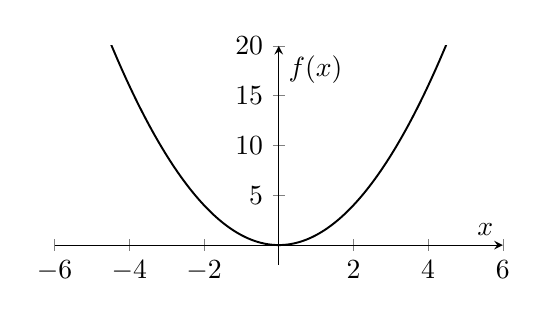
\begin{tikzpicture}
\begin{axis}[
  width=0.6\textwidth, height=0.36\textwidth,
  axis lines=middle,
  xmin=-6, xmax=6, ymin=-2, ymax=20,
  samples=250, domain=-6:6,
  xlabel={$x$}, ylabel={$f(x)$}
]
\addplot[black, line width=0.7pt] {x^2};
\end{axis}
\end{tikzpicture}
\caption{A quadratic: $f(x)=x^2$.}
\end{figure}

% ------------------------------------------------------------
\subsection{The exponential function}

\[
f(x)=e^x.
\]

\textbf{Properties:} always positive, strictly increasing, derivative equals itself.

\textbf{Uses:} population growth, compound interest, differential equations.

\begin{figure}[h]
\centering
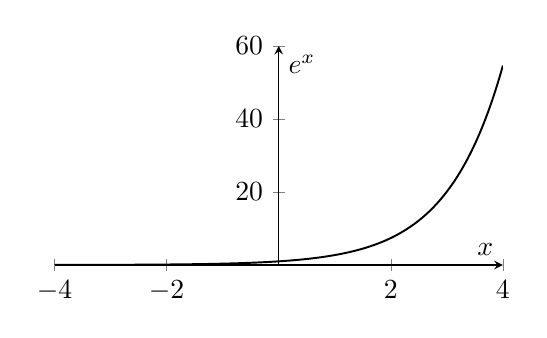
\begin{tikzpicture}
\begin{axis}[
  width=0.6\textwidth, height=0.36\textwidth,
  axis lines=middle,
  xmin=-4, xmax=4, ymin=0, ymax=60,
  samples=250, domain=-4:4,
  xlabel={$x$}, ylabel={$e^x$}
]
\addplot[black, line width=0.7pt] {exp(x)};
\end{axis}
\end{tikzpicture}
\caption{Exponential growth: $f(x)=e^x$.}
\end{figure}

% ------------------------------------------------------------
\subsection{The negative exponential}

\[
f(x)=e^{-x}.
\]

\textbf{Properties:} positive, strictly decreasing, approaches $0$ as $x\to\infty$.

\textbf{Uses:} radioactive decay, discounting, cooling.

\begin{figure}[h]
\centering
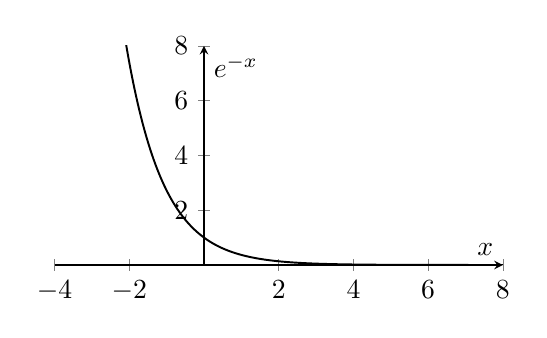
\begin{tikzpicture}
\begin{axis}[
  width=0.6\textwidth, height=0.36\textwidth,
  axis lines=middle,
  xmin=-4, xmax=8, ymin=0, ymax=8,
  samples=250, domain=-4:8,
  xlabel={$x$}, ylabel={$e^{-x}$}
]
\addplot[black, line width=0.7pt] {exp(-x)};
\end{axis}
\end{tikzpicture}
\caption{Exponential decay.}
\end{figure}

% ------------------------------------------------------------
\subsection{The logarithm}

\[
f(x)=\ln x,\qquad x>0.
\]

\textbf{Properties:} strictly increasing, slow growth, inverse of $e^x$.

\textbf{Uses:} multiplicative-to-additive conversion, data compression, statistics.

\begin{figure}[h]
\centering
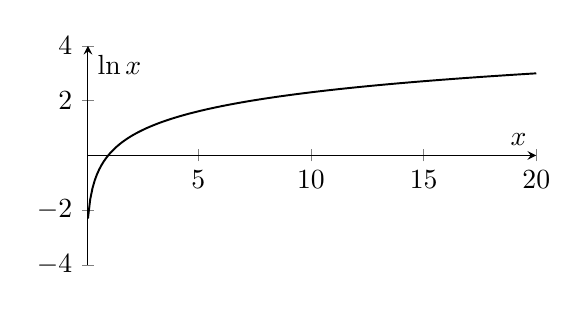
\begin{tikzpicture}
\begin{axis}[
  width=0.6\textwidth, height=0.36\textwidth,
  axis lines=middle,
  xmin=0.1, xmax=20, ymin=-4, ymax=4,
  samples=200, domain=0.1:20,
  xlabel={$x$}, ylabel={$\ln x$}
]
\addplot[black, line width=0.7pt] {ln(x)};
\end{axis}
\end{tikzpicture}
\caption{Logarithmic growth: $f(x)=\ln x$.}
\end{figure}

% ------------------------------------------------------------
\subsection{The sinusoid}

\[
f(x)=\sin x.
\]

\textbf{Properties:} periodic, oscillatory, bounded, smooth.

\textbf{Uses:} waves, AC electricity, tides, Fourier series.

\begin{figure}[h]
\centering
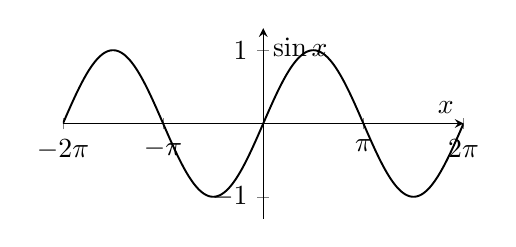
\begin{tikzpicture}
\begin{axis}[
  width=0.55\textwidth, height=0.33\textwidth,
  axis lines=middle,
  xmin=-2*pi, xmax=2*pi, ymin=-1.3, ymax=1.3,
  samples=300, domain=-2*pi:2*pi,
  xlabel={$x$}, ylabel={$\sin x$},
  xtick={-6.28318,-3.14159,0,3.14159,6.28318},
  xticklabels={$-2\pi$,$-\pi$,0,$\pi$,$2\pi$}
]
\addplot[black, line width=0.7pt] {sin(deg(x))};
\end{axis}
\end{tikzpicture}
\caption{A sinusoidal oscillation: $f(x)=\sin x$.}
\end{figure}

% ------------------------------------------------------------
\subsection{The Gaussian (normal curve)}

\[
f(x)=\frac{1}{\sqrt{2\pi}}\,e^{-x^2/2}.
\]

\textbf{Properties:} symmetric, bell-shaped, rapidly decaying tails.

\textbf{Uses:} measurement error, statistics, noise modelling.

\begin{figure}[h]
\centering
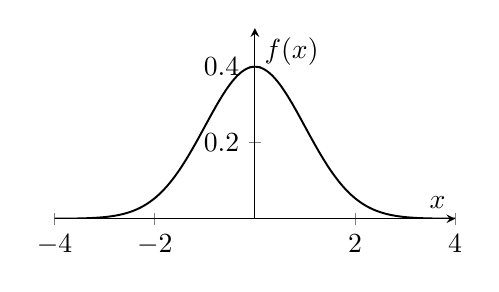
\begin{tikzpicture}
\begin{axis}[
  width=0.55\textwidth, height=0.33\textwidth,
  axis lines=middle,
  xmin=-4, xmax=4, ymin=0, ymax=0.5,
  samples=250, domain=-4:4,
  xlabel={$x$}, ylabel={$f(x)$}
]
\addplot[black, line width=0.7pt] {1/sqrt(2*pi)*exp(-x^2/2)};
\end{axis}
\end{tikzpicture}
\caption{Standard Gaussian density.}
\end{figure}

% ------------------------------------------------------------
\subsection{The logistic function}

\[
f(x)=\frac{1}{1+e^{-x}}.
\]

\textbf{Properties:} S-shaped, bounded, symmetric about $x=0$.

\textbf{Uses:} constrained growth, technology adoption, logistic regression.

\begin{figure}[h]
\centering
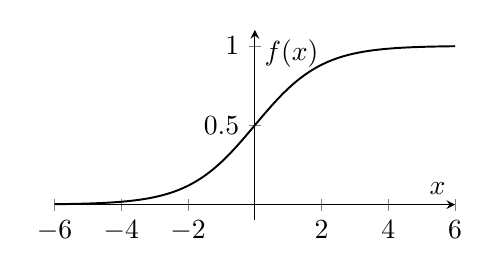
\begin{tikzpicture}
\begin{axis}[
  width=0.55\textwidth, height=0.33\textwidth,
  axis lines=middle,
  xmin=-6, xmax=6, ymin=-0.1, ymax=1.1,
  samples=250, domain=-6:6,
  xlabel={$x$}, ylabel={$f(x)$}
]
\addplot[black, line width=0.7pt] {1/(1+exp(-x))};
\end{axis}
\end{tikzpicture}
\caption{Logistic (saturation) curve.}
\end{figure}

% ------------------------------------------------------------
\subsection*{A closing remark}

These functions recur because each captures a deep ``shape'' that nature and
society repeatedly exhibit: quadratic curvature, exponential growth and decay,
logarithmic compression, sinusoidal oscillation, Gaussian randomness, and
logistic saturation.  Learning their properties is like acquiring a small but
powerful vocabulary for the real world.
%%%%%%%%%%%%%%%%%%%%%%%%%%%%%%%%%%%%%%%%%%%%%%%%%%%%%%%%%%%%%%
\section*{Summary}

The real numbers complete the rationals, resolve ancient paradoxes, and support the modern theory of limits, continuity, and calculus. They underpin geometry, physics, finance, and modelling, and form the domain for the most important functions in science. Understanding real numbers is therefore a gateway into nearly every field of mathematics and its applications.

\section*{Problems}

\begin{enumerate}

% ------------------------------
\item (\textbf{Arithmetic sequences})
An arithmetic progression has first term $a$ and common difference $d$.
Show that the average of the first $n$ terms equals the average of the first and $n$th terms.
Use this fact to re-derive the sum formula $S_n = \frac{n}{2}(2a + (n-1)d)$.

% ------------------------------
\item (\textbf{Geometric growth})
A bacteria culture triples every hour.
If it starts with $B_0$ bacteria at time $t=0$, express $B_t$ as a geometric progression.
How long does it take to exceed $50\,B_0$?

% ------------------------------
\item (\textbf{Polynomial addition and multiplication})
Let 
\[
p(x)=3x^3-2x+7,\qquad q(x)=x^2-4.
\]
Compute $p(x)+q(x)$ and $p(x)\cdot q(x)$ and state their degrees.
Explain why degrees add under multiplication.

% ------------------------------
\item (\textbf{Decimal as a polynomial})
Interpret the decimal number $40756$ as a polynomial in $10$
evaluated at $10$.  
Rewrite it using powers of $2$ instead of $10$ by expanding it in base $2$.

% ------------------------------
\item (\textbf{Interpolation})
Given three points $(0,1)$, $(1,3)$, $(2,6)$:
\begin{enumerate}
    \item Construct the Lagrange basis polynomials $L_0(x)$, $L_1(x)$, $L_2(x)$.
    \item Write down the interpolating polynomial explicitly.
    \item Evaluate it at $x = 1/2$.
\end{enumerate}

% ------------------------------
\item (\textbf{Overfitting with polynomials})
Explain why there always exists a polynomial of degree $n-1$
passing through $n$ given data points,
but why such a polynomial might be a poor model for prediction.

% ------------------------------
\item (\textbf{Linear regression intuition})
Consider the data points $(0,3)$, $(1,2)$, $(2,2)$, $(3,5)$.
Sketch a line that “best fits’’ the data by eye.
Explain qualitatively why the least-squares line minimises the sum of squared vertical errors.

% ------------------------------
\item (\textbf{Systems of equations})
Solve the system:
\[
\begin{cases}
3x + y = 7,\\
2x - y = 1.
\end{cases}
\]
Then interpret the solution as the intersection of two lines.

% ------------------------------
\item (\textbf{Linearity in modelling})
A factory produces two products $A$ and $B$.
Each unit of $A$ requires $2$ hours of machine time and $3$ units of raw material.
Each unit of $B$ requires $1$ hour of machine time and $4$ units of raw material.
If the factory uses $23$ hours of machine time and $41$ units of raw material in total,
set up the linear system and solve for the production quantities.

% ------------------------------
\item (\textbf{Uniqueness of solutions})
Give an example of a $2\times 2$ linear system with:
\begin{itemize}
    \item exactly one solution,
    \item infinitely many solutions,
    \item no solution.
\end{itemize}
Explain geometrically why these cases correspond to
intersecting lines, coincident lines, and parallel lines.

% ------------------------------
\item (\textbf{Function families})
For each of the functions below—quadratic, exponential, logarithmic,
sinusoidal, logistic—provide:
\begin{enumerate}
    \item a real-world phenomenon it models,
    \item whether it is increasing, decreasing, periodic, or saturating,
    \item the effect of scaling the input (e.g.\ replacing $x$ by $kx$).
\end{enumerate}

% ------------------------------
\item (\textbf{Gaussian decay})
Show that the Gaussian function
\[
g(x)=e^{-x^2}
\]
decays faster than any exponential $e^{-c x}$ as $x\to\infty$.
(Hint: compare exponents.)

\end{enumerate}
